
\chapter{Chapter 2 Supplemental Information}
\label{sec:app2}
\raggedbottom


%%%%%%%%%%%%%%%%%%%%%%%%%%%

%%%%%%%%%%%%%%%%%%%%%%%%%%%_________________CHAPTERTWO_________________%%%%%%%%%%%%%%%%%%%%%%%%%%%

%%%%%%%%%%%%%%%%%%%%%%%%%%%
\clearpage
\section{Supplemental Figures}
%Supplemental Figure 1: Histogram of TPM distribution
\begin{figure}[h!]
  \centering
    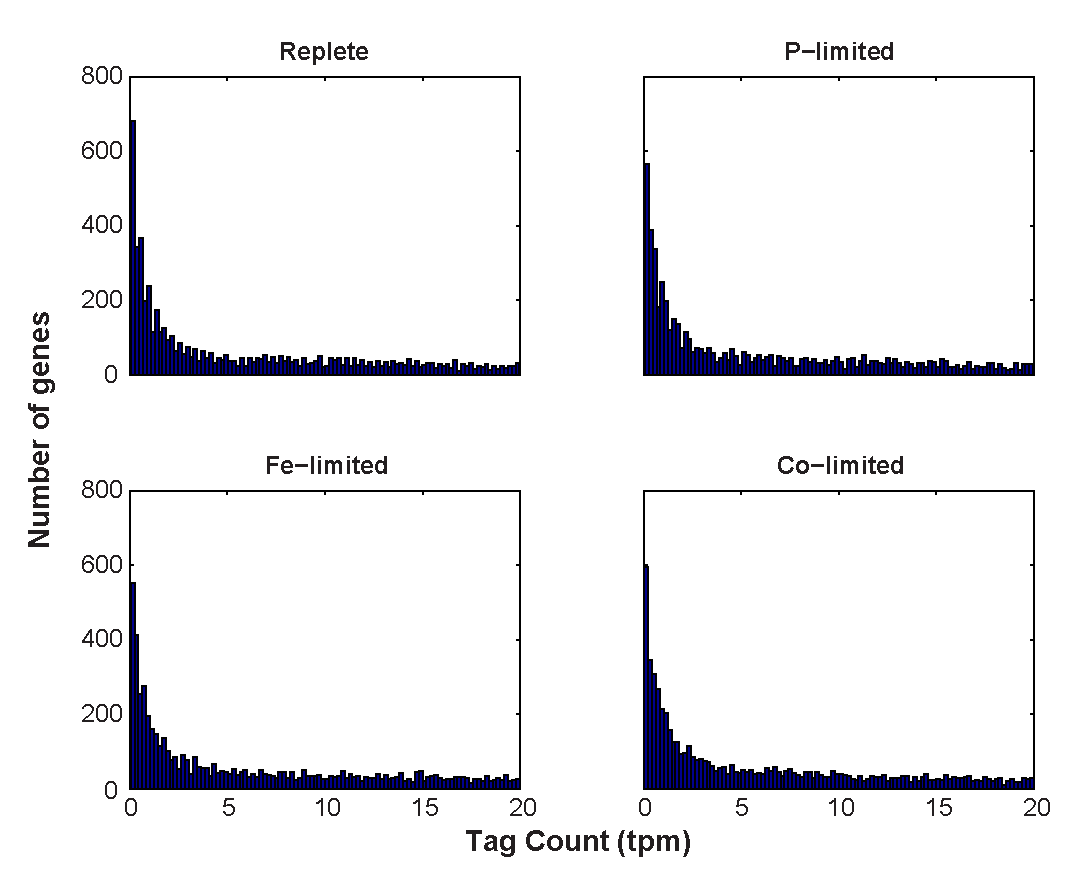
\includegraphics[width=1\textwidth]{Images/C2_FigureS1_v6.pdf}
    \caption[Distribution of normalized tag counts across treatments]{Histogram analysis of the distribution of normalized tag counts (TPM) for each gene across each of the four treatments (Replete, P-limited, Fe-limited, and co-limited). The abundance of normalized tag counts (TPM) was assessed, tallying the total number of genes with a given tag count. Only tag counts less than 20 are depicted to aid the visualization of the inflection in the data at 2.5 TPM.}
  \label{fig:a1f1}
\end{figure}

%Supplemental Figure 2: K-means clusters (all)
\begin{landscape}
   \null         %%<---- this is needed
   \vfill        %%<-----here
   \centering 
    \begin{figure}
    \centering
        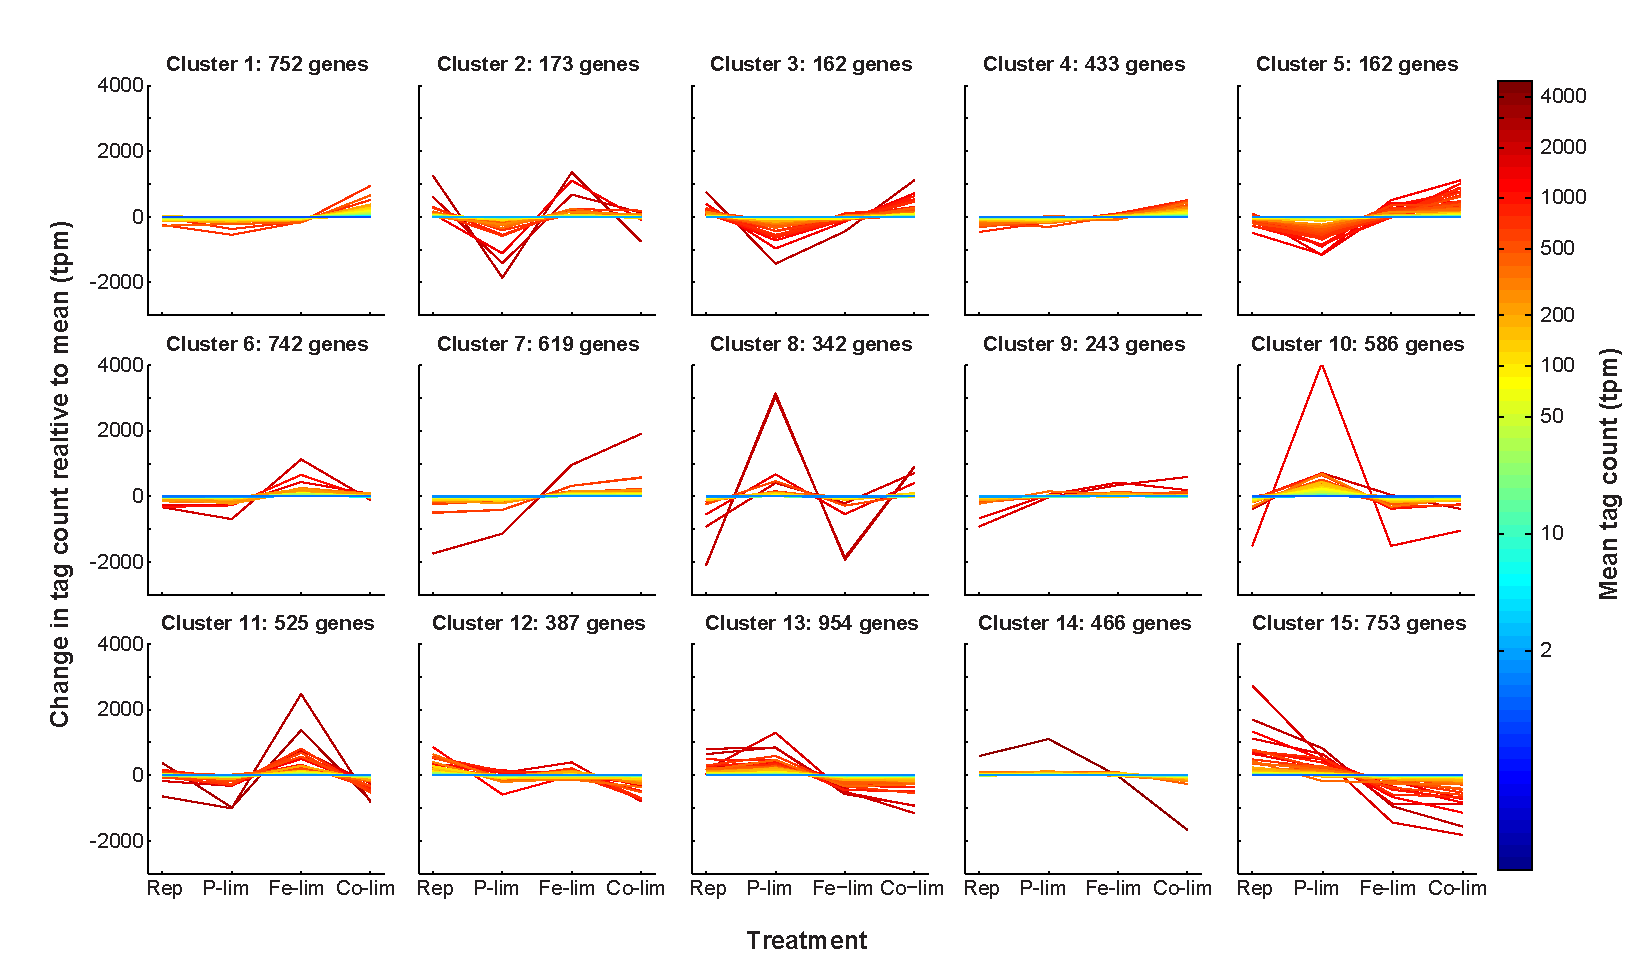
\includegraphics[width=1\textwidth]{Images/C2_FigureS2_v6.pdf}
        \caption[$K$-means clustering of normalized genes]{$K$-means clustering of normalized genes. The 7380 genes that passed the 2.5 TPM cutoff were clustered into 15 clusters using the $k$-means algorithm under the Pearson correlation coefficient. Tag counts normalized to total library size (in TPM) for each gene are plotted relative to the mean (indicated by the color of the line) for each of the four treatments: Replete (Rep), P-limited (P-lim), Fe-limited (Fe-lim), and co-limited (Co-lim).}
  \label{fig:a1f2}

    \end{figure}
    \vfill        %%<----- and here
\end{landscape}

\clearpage
\section{Supplemental Data}


    \begin{DS2}
    
    \item \label{DS21}: Genes in the \textit{T. pseudonana} genome homologous to reference genes from relative expression studies in algae and plants. \href{http://journal.frontiersin.org/file/downloadfile/16019/octet-stream/Data\%20Sheet\%201.XLS/313/2/31186}{Data Sheet 2-1} can be downloaded from the online version of the manuscript of \citet{Alexander2012} through \href{http://dx.doi.org/10.3389/fmicb.2012.00385}{Frontiers in Aquatic Microbiology}. 
    \item \label{DS22}: Putative reference genes identified with k-means clustering analysis (Cluster 9 and Clusters 14). \href{http://journal.frontiersin.org/file/downloadfile/16022/octet-stream/Data\%20Sheet\%202.XLS/313/1/31186}{Data Sheet 2-2} can be downloaded from the online version of the manuscript of \citet{Alexander2012} through \href{http://dx.doi.org/10.3389/fmicb.2012.00385}{Frontiers in Aquatic Microbiology}. 
        \item \label{DS23}: Data Sheet 3. Putative reference genes identified with ASC analysis ($p < 0.1$ for a fold change of 1.25). \href{http://journal.frontiersin.org/file/downloadfile/16025/octet-stream/Data\%20Sheet\%203.XLS/313/1/31186}{Data Sheet 2-3} can be downloaded from the online version of the manuscript of \citet{Alexander2012} through \href{http://dx.doi.org/10.3389/fmicb.2012.00385}{Frontiers in Aquatic Microbiology}. 

            \item \label{DS24}: The intersection of differentially expressed genes identified by \citet{Mock2008} and stably expressed genes identified through ASC (1.25 fold change bin, $p < 0.1$). \href{http://journal.frontiersin.org/file/downloadfile/16028/octet-stream/Data\%20Sheet\%204.XLS/313/1/31186}{Data Sheet 2-4} can be downloaded from the online version of the manuscript of \citet{Alexander2012} through \href{http://dx.doi.org/10.3389/fmicb.2012.00385}{Frontiers in Aquatic Microbiology}. 

    \end{DS2}




